\section{Grundlagen}


\subsection{Definitionen} \label{Definitionen}
Um Reinforcement Learning im Folgenden besser beschreiben zu können, ist zunächst die Klärung einiger Grundbegriffe nötig. Diese sind aus der englischen Sprache entstanden, auf eine Übersetzung dieser Begriffe in das Deutsche wurde verzichtet, um eine Vergleichbarkeit zu anderen Werken in diesem Themenbereich zu gewährleisten.

\begin{enumerate}
    \item \textbf{Markov Decision Process}\\
    Ein Markov Decision Process (MDP) \cite{builtinUnderstandingMarkov} ist ein formales Modell, das zur Beschreibung von Entscheidungsproblemen verwendet wird, bei denen eine Entscheidungsträgerin oder ein Entscheidungsträger (oft als Agent bezeichnet) in einer Umgebung handelt und dabei versucht, eine bestimmte Zielsetzung zu erreichen. Ein MDP basiert auf dem Konzept eines Markov-Prozesses, der ein stochastischer Prozess ist, bei dem der zukünftige Zustand nur vom gegenwärtigen Zustand abhängt und nicht von früheren Zuständen.

    Ein MDP besteht aus den folgenden Komponenten:

    \begin{enumerate}
        \item \textit{Agent}\\
        Der Agent \cite{mediumBeginnersGuide} ist der Entscheidungsträger, welcher Aktionen in einem Szenario/Umfeld ausführt und dafür eine Belohnung bekommt.
        \item \textit{Environment}\\
        Das Environment \cite{datasolutReinforcementLearning} ist, wie die deutsche Übersetzung schon vermutet lässt, die Umgebung in dem sich der Agent befindet. Das Environment legt dabei die grundlegenden Regeln fest und definiert, welche Aktionen möglich sind. Das Environment trägt somit ausschlaggebend zur Komplexität der zu lösenden Aufgabe bei. In vielen Fällen, so auch in den in dieser Ausarbeitung folgenden Versuchen, ist das Environment eine Simulation. Dies ermöglicht einen deutlich schnelleren Lernprozess, da jegliche Interaktion ohne nennenswerte Verzögerung ausgeführt werden kann. Bei komplexen Aufgabestellungen ist es so zudem möglich, mehrere Agenten parallel zu trainieren.
        \item \textit{Action}\\
        Als Action \textbf{\textit{A}} wird eine Interaktion des Agent mit dem Environment beschrieben. Die Lösung eines Problems kann somit als Abfolge bestimmter Actions angesehen werden. Welche Actions der Agent ausführen kann, hängt dabei von den Grundregeln des Environments ab.
        \item \textit{State}\\
        Der State \textbf{\textit{S}} ist der eindeutige und vollständige Beschreibung des Zustands, in welchem sich das Environment befindet. Aus technischer Sicht ist der State meist ein Vektor, eine Matrix und ein Tensor, welcher alle relevanten Information des aktuellen Zustands enthält.
        \item \textit{Reward}\\
        Der Reward \textbf{\textit{R}} \cite{datasolutReinforcementLearning} ist die unmittelbare Belohnung, welche der Agent als Feedback zu einer Action erhält. In der Praxis ist dies ein numerischer Wert, welche entweder erhöht oder reduziert werden kann. Der Agent kann so für eine Action belohnt oder bestraft werden, dabei versucht er sein Handeln so auszurichten, dass er die größte mögliche Belohnung erreicht. Die Art und Weise, wie der Reward vergeben wird, bestimmt somit das Verhalten des Agents.
    \end{enumerate}

    Das Ziel des Agenten in einem MDP besteht darin, eine Strategie zu entwickeln, die ihm dabei hilft, die maximale kumulierte Belohnung im Laufe der Zeit zu erhalten. Eine Strategie ist eine Abbildung von Zuständen auf Aktionen, die angibt, welche Aktion der Agent in jedem Zustand ausführen sollte. Die optimale Strategie maximiert die erwartete zukünftige Belohnung über alle Zustände und Aktionen.
    
    Der MDP besitzt, wie eben beschrieben, eine Menge an States \textbf{\textit{S}}, eine Menge an Aktionen \textbf{\textit{A}} und eine Menge an \textbf{\textit{R}}.
    In dem Prozess werden die Schritte \textbf{\textit{t} = 0,1,2,...} durchlaufen und der Agent befindet sich jeweils in einem State $ \text{\textbf{\textit{S\textsubscript{t}}}}\in \text{\textbf{\textit{S}}}$. 
    Basierend auf diesem State kann der Agent eine Action $ \text{\textbf{\textit{A\textsubscript{t}}}}\in \text{\textbf{\textit{A}}}$ wählen. Dies ergibt dann das State-Action Paar (\textbf{\textit{S\textsubscript{t}}}, \textbf{\textit{A\textsubscript{t}}}).

    In dem nächsten Schritt \textbf{\textit{t} + 1} wird das Environment in den State $ \text{\textbf{\textit{S\textsubscript{t+1}}}}\in \text{\textbf{\textit{S}}}$ überführt.
    Hier bekommt der Agent nun den entsprechenden Reward $ \text{\textbf{\textit{R\textsubscript{t+1}}}}\in \text{\textbf{\textit{R}}}$ für die Action \textbf{\textit{A\textsubscript{t}}},
    welcher er zuvor in State \textbf{\textit{S\textsubscript{t}}} genommen hat. Dieser Prozess ist in der Abbildung \ref{MDP} abgebildet.


    \begin{figure}
        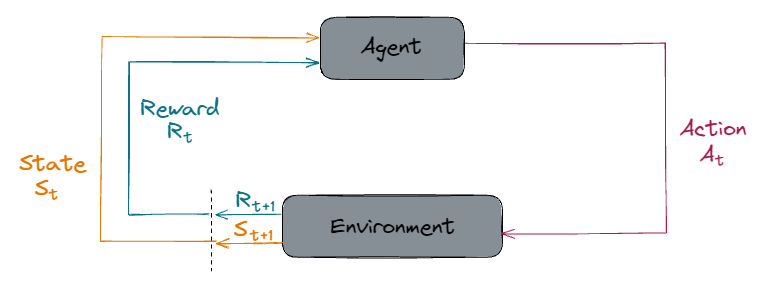
\includegraphics[scale=0.7]{MDP}
        \caption{Markov Decision Process}
        \label{MDP}
    \end{figure}
    \item \label{itm:Episode} \textbf{Episode} \\
    Als Episode \cite{lesswrongWhatTraining} wird ein vollständiger Durchlauf während des Trainings bezeichnet. Jede Episode startet mit dem Anfangszustand des Environments und kann auf mehreren Wegen enden. Im besten Fall wird die Episode beendet, weil die gestellte Aufgabe vom Agent gelöst worden ist. In vielen Fällen wird eine Episode jedoch abgebrochen, weil die maximale Anzahl an Actions überschritten wurde. Eine solche Grenze wird implementiert, um sicherzustellen, dass das Training effektiv und effizient abläuft. Wenn keine Obergrenze festgelegt wird, kann der Agent endlos versuchen, das Ziel zu erreichen, ohne jemals erfolgreich zu sein. Zudem kann so verhindert werden, dass der Agent in einer Schleife von kleinen Belohnungen feststeckt. Die letzte Möglichkeit, wie eine Episode enden kann, ist von Environment definiert, in vielen Fällen kann der Agent durch bestimmte Fehlentscheidungen die Episode beendet.
    
    \item \textbf{Policy}\\
    Im Reinforcement Learning bezeichnet eine Policy {$\bm{\pi}$} \cite{mediumReinforcementLearningPolicyValue} eine Funktion, die Entscheidungen trifft, um eine bestimmte Aufgabe zu lösen. Eine Policy entscheidet, welche Aktion ein Agent in einer bestimmten Situation ausführen soll, basierend auf den Informationen, die der Agent in der Vergangenheit gesammelt hat.

    Die Policy wird durch das Optimierungsproblem des Reinforcement Learning bestimmt, das darin besteht, die optimale Strategie zu finden, um die Belohnung des Agents zu maximieren. Die optimale Policy ist diejenige, die in jeder Situation die Aktion empfiehlt, die die höchste erwartete Belohnung ergibt.

    Es gibt verschiedene Arten von Policies im Reinforcement Learning, wie beispielsweise deterministische Policies, stochastische Policies und epsilon-greedy Policies. Eine deterministische Policy gibt für jede Situation genau eine Aktion vor, während eine stochastische Policy eine Wahrscheinlichkeitsverteilung über alle Aktionen in einer Situation bereitstellt. Die epsilon-greedy Policy ist eine Mischung aus deterministischen und stochastischen Policies und wählt die Aktion mit der höchsten erwarteten Belohnung mit einer Wahrscheinlichkeit von 1-epsilon und eine zufällige Aktion mit einer Wahrscheinlichkeit von epsilon aus.
    
    \item \textbf{Value Function}\\
    Bei dem Begriff Value Function \cite{mediumReinforcementLearningPolicyValue} handelt es sich um eine eine Funktion, die den erwarteten Wert einer bestimmten State-Action-Kombination oder eines States wiedergibt. Der Wert gibt an, wie nützlich es ist, sich in diesem State oder dieser Kombination zu befinden, um das Gesamtziel zu erreichen, also die maximale Belohnung zu erhalten.

    Die Value Function kann verwendet werden, um die optimale Policy zu finden, die die maximale Belohnung im Laufe der Zeit liefert. In Reinforcement Learning gibt es zwei Arten von Value Functions: Die State-Value Function und die Action-Value Function.
    
    Die State-Value Function \textbf{\textit{V}} gibt den erwarteten Wert der Gesamtbelohnungen an, den ein Agent in einem bestimmten Zustand erzielen kann. Mit anderen Worten, sie gibt an, wie nützlich es ist, sich in einem bestimmten Zustand zu befinden, um das Ziel der maximalen Belohnung zu erreichen. Die Zustandswertfunktion wird oft als \textbf{\textit{V(s)}} bezeichnet, wobei s der Zustand ist.
    
    Die Action-Value Function \textbf{\textit{Q}} gibt den erwarteten Wert des Gesamtbelohnungen an, den ein Agent in einem bestimmten Zustand erreichen kann, wenn er eine bestimmte Aktion ausführt. Mit anderen Worten, sie gibt an, wie nützlich es ist, in einem bestimmten Zustand eine bestimmte Aktion auszuführen. Die Aktionswertfunktion wird oft als \textbf{\textit{Q(s,a)}} bezeichnet, wobei s der Zustand und a die Aktion sind.
    
    Value Functions können auf verschiedene Weise geschätzt werden, wie z.B. mit Hilfe von Monte-Carlo-Methoden und Temporal Difference Learning.

    Im weiteren Verlauf der Arbeit wurde sich mit der Action-Value Function \textbf{\textit{Q}} und dem Temporal Difference Learning auseinandergesetzt.
    
    \item \textbf{Temporal Difference Learning}\\
    Temporal Difference (TD) Learning \cite{mediumTemporalDifference} ist eine Methode des Reinforcement Learning, die es einem Agenten ermöglicht, aus Erfahrungen zu lernen, indem er die erzielte Belohnung mit der erwarteten Belohnung vergleicht. Im Gegensatz zu Monte-Carlo-Methoden, die die Gesamtrabatte aus der Erfahrung berechnen, werden bei TD-Learning die Value Functions schrittweise durch den Vergleich von aufeinanderfolgenden Schätzungen aktualisiert.

    Die TD-Learning Methode verwendet dabei die Bellman-Gleichungen, um die Value Functions zu aktualisieren. Diese Gleichungen sind eine Reihe von Gleichungen, die die Beziehung zwischen den Zustands- und Aktionswerten und der optimalen Policy beschreiben.

    Wenn der Agent eine Aktion ausführt und in einen neuen Zustand gelangt, wird die erhaltene Belohnung zusammen mit dem geschätzten zukünftigen Wert des nächsten Zustands verwendet, um eine neue Schätzung der Value Function zu berechnen. Diese Schätzung wird dann mit der vorherigen Schätzung der Value Function kombiniert, um die Value Function schrittweise zu aktualisieren.

    Im TD-Learning gibt es zwei wichtige Methoden: SARSA (State-Action-Reward-State-Action) und Q-Learning.

    \item \textbf{Optimalität}\\
    \begin{enumerate}
        \item \textit{Optimale Policy}\\
        Das Ziel beim Reinforcement Learning ist es, eine Policy {$\bm{\pi}$} zu finden, welche die Belohnung des Agenten maximiert. Dafür muss die Policy {$\bm{\pi}$} gefunden werden, welche dem Agenten mehr Belohnung liefert, als jede andere Policy {$\bm{\pi'}$}.
        
        Mathematisch formuliert muss folgendes gelten:

        \begin{align}
            \bm{\pi} \geq \bm{\pi'}\text{ if } q_{\pi}(s,a) \geq  q_{\pi'}(s,a)\text{ for all } s \in S \text{ and } a \in A
        \end{align}

        Hierbei ist $q_{\pi}(s,a)$ die Action-Value Function, welche der optimalen Policy {$\bm{\pi}$} folgt.

        \item \textit{Optimale Action-Value Function}\\
        Für die optimale Action-Value Function gilt folgende Gleichung $\bm{q_{*}}$:

        \begin{align}
            q_{*}(s,a)=\max_{\pi}q_{\pi}(s,a)
        \end{align}
    
        Somit liefert $\bm{q_{*}}$ die größten erwarteten Belohnungen für jede Policy {$\bm{\pi}$} für jedes mögliche State-Action Paar.


        \item \textit{Bellman Optimality Equation}\\
        Die Bellman Optimality Equation \cite{floydhubIntroductionQLearning} für die Action-Value Function beschreibt den optimalen Wert eines State-Action Paares \textbf{\textit{(s,a)}} unter der Annahme, dass der Agent die optimale Policy verfolgt.

        \begin{align}
        q_{*}(s,a)=E[R_{t+1}+\gamma \max_{a'} q_{*}(s', a')]
        \end{align}

        Sie kann genutzt werden um in einem iterativen Prozess die optimale Action-Value Function $\bm{q_{*}}$ zu finden.
    \end{enumerate}

    
    \item \textbf{Exploration vs Exploitation} \label{ExpvsExp}\\
    Exploration \cite{towardsdatascienceExplorationReinforcement} bezieht sich auf die Strategie des Agents, neue Entscheidungen zu erkunden und zu lernen, indem er Aktionen ausprobiert, die er noch nicht ausprobiert hat. Der Agent versucht, neue Möglichkeiten zu erforschen, um mehr über die Umgebung zu erfahren.

    Exploitation hingegen bezieht sich auf die Strategie des Agents, Entscheidungen auf der Grundlage der bisherigen Erfahrungen zu treffen, um den maximalen Gewinn zu erzielen. Mit anderen Worten, der Agent nutzt die bisherigen Erfahrungen, um die Aktion auszuwählen, die ihm die höchste Belohnung in der Vergangenheit gegeben hat.
    
    Ein Gleichgewicht zwischen Exploration und Exploitation ist wichtig, um optimale Entscheidungen zu treffen. Wenn der Agent zu sehr auf Exploration setzt, wird er immer wieder neue Entscheidungen ausprobieren und keine optimale Entscheidung treffen, um den maximalen Gewinn zu erzielen. Wenn der Agent hingegen zu sehr auf Exploitation setzt, wird er sich auf die Entscheidungen konzentrieren, die ihm in der Vergangenheit den höchsten Gewinn gebracht haben, und nicht in der Lage sein, neue Entscheidungen zu erkunden, die möglicherweise noch höhere Gewinne erzielen können.
    
    Daher verwenden Reinforcement Learning-Algorithmen oft eine Strategie namens epsilon-greedy-Strategie, bei der der Agent mit einer Wahrscheinlichkeit von epsilon eine zufällige Aktion auswählt, um Exploration durchzuführen, und mit einer Wahrscheinlichkeit von 1 - epsilon eine Aktion auswählt, die bisher die höchste Belohnung erzielt hat, um Exploitation durchzuführen. Auf diese Weise kann der Agent gleichzeitig erkunden und von seinen bisherigen Erfahrungen profitieren, um optimale Entscheidungen zu treffen.

\end{enumerate}

\subsection{Algorithmen}

\subsubsection{Q-Learning}

Q-Learning ist ein iteratives, modellfreies Reinforcement Learning Verfahren aus dem Bereich der Temporal Difference Learning Verfahren, das verwendet wird, um die optimale Action-Value Functon $\bm{Q_{*}(s,a)}$ zu lernen, indem es Erfahrungen sammelt und die Action-Values iterativ aktualisiert.

Das Verfahren basiert auf der Bellman Optimality Equation für die Action-Value Function $\bm{Q_{*}(s,a)}$, die besagt, dass der optimale Wert eines State-Action Paars $\bm{(s,a)}$ die maximale erwartete zukünftige Belohnung ist, die durch die Wahl der optimalen Actions in diesem State und danach unter Verwendung der optimalen Policy erreicht wird.

Q-Learning nutzt eine Tabelle, die die Values für jedes State-Action Paar $\bm{(s,a)}$ speichert. Das Verfahren sammelt Erfahrungen, indem es den Agenten in der Umgebung handeln lässt, und verwendet diese Erfahrungen, um die Values zu aktualisieren. Die Aktualisierung erfolgt durch die Formel:


\begin{align}
    Q(s,a) \leftarrow Q(s,a) + \alpha [R + \gamma \max_{a'} Q(s',a') - Q(s,a)]
\end{align}


wobei $\bm{Q(s,a)}$ das aktuelle Value für das State-Action Paar $\bm{(s,a)}$ ist, $\bm\alpha$ die Learning Rate ist, $\bm{R}$ die unmittelbare Belohnung ist, $\bm\gamma$ die Discount Rate ist, die die zukünftige Gesamtbelohnung gewichtet, und $\bm{\max_{a'} Q(s',a')}$ die erwartete zukünftige Gesamtbelohnung ist, die durch Wahl der optimalen Action $\bm{a'}$ im nächsten Zustand $\bm{s'}$ erreicht wird.

Der Agent verwendet eine Exploration-Exploitation Strategie, um die Umgebung zu erkunden und gleichzeitig die bereits bekannten Informationen zu nutzen. Die Exploration wird durch zufällige Actions gesteuert, während die Exploitation durch die Wahl der Actions mit den höchsten Action-Value erreicht wird.



\subsubsection{SARSA}

Ähnlich wie bei Q-Learning basiert SARSA auf der Bellman Optimality Equation, aber im Gegensatz zu Q-Learning lernt SARSA direkt die Aktionswerte der Policy, die tatsächlich ausgeführt wird. Dies bedeutet, dass SARSA bei der Aktualisierung der Action-Values die nächste Action $\bm{a'}$ basierend auf der aktuellen Policy wählt, anstatt die Action mit dem höchsten Action-Value zu wählen, wie dies bei Q-Learning der Fall ist.
Daher spricht man bei Q-Learning auch von einem off-Policy Algorithmus, während SARSA ein on-Policy Algorithmus ist. 

Die Aktualisierungsregel von SARSA ist wie folgt:

\begin{align}
    Q(s,a) \leftarrow Q(s,a) + \alpha [R + \gamma Q(s',a') - Q(s,a)]
\end{align}

wobei der Unterschied in dem Term $\gamma Q(s',a')$ liegt. Denn hierbei wird wieder das epsilon-greedy Verfahren benutzt um den Action-Value zu bestimmen, im Vergleich zu dem maximalen Value, welcher bei Q-Learning gewählt wurde.

\subsection{Hyperparameter}\label{Def_Hyperparameter}
Unter Hyperparametern versteht man Einstellungen oder Konfigurationen für einen Maschine-Learning-Algorithmus, um das Verhalten und die Leistung zu steuern. Diese werden vor Beginn des Trainings festgelegt. Da die Wahl der Hyperparameter einen großen Einfluss auf die Fähigkeit der Modelle hat, ist es für den späteren Vergleich wichtig diese Parameter für jeden Algorithmus zu optimieren, um einen fairen Vergleich gewährleisten zu können.
\begin{itemize}
    \item \textbf{Anzahl an Episoden}\\
    Wie bereits bei \ref*{Definitionen} \nameref{itm:Episode} beschrieben, stellt eine Episode einen vollständigen Durchlauf des Environments dar. Die Anzahl dieser Durchläufe währende des Trainingsprozesses wird als Hyperparameter festgelegt. Umso mehr Durchläufe der Agent zur Verfügung hat, um so häufiger kann er dazulernen und sich anpassen, somit hat dieser Hyperparameter einen großen Einfluss auf die Leistung des Agent. Die Anzahl der Episoden steht zudem im direkten Zusammenhang zu der für das Training benötigte Zeit, umso mehr Episoden durchlaufen werden, umso länger dauert der gesamte Trainingsprozess. Die optimale Anzahl der Episoden hängt von verschiedenen Faktoren wie der Komplexität der Umgebung, der Anzahl der States sowie dem verwendeten Lernalgorithmus ab. Bei zu wenigen Episoden ist der Algorithmus nicht in der Lage sein volles Potenzial zu entfalten. Zu viele Episoden können, besonders bei komplexen Modellen, zu Overfitting führen, dabei lernt der Agent die Umgebung auswendig und kann so nicht auf neue Situationen reagieren.
    \item \textbf{Discount Faktor}\\
    Der Discount Faktor bestimmt, wie stark der Agent eine Belohnung in der Zukunft gewichtet im Vergleich zu einer sofortigen Belohnung. Ein höherer Discount-Faktor bedeutet, dass der Agent die zukünftigen Belohnungen stärker gewichtet und daher eher langfristige Entscheidungen trifft. Ein niedrigerer Discount-Faktor führt dagegen zu kurzfristigeren Entscheidungen, da zukünftige Belohnungen weniger stark gewichtet werden. Der Wertebereich für diesen Hyperparameter liegt zwischen null und eins. Im ersten Moment könnte man jetzt denken, dass der höchstmögliche Discount Faktor der beste sei, da so der komplette Fokus auf dem Endergebnis der Episode liegt. Dies ist aber in den meisten Fällen nicht korrekt. Denn nicht jede Entscheidung hat einen Effekt, der bis zum Ende der Episode reicht, der Agent wäre dann nicht in der Lage solche Entscheidungen zu treffen. Zudem würden bei jeder Entscheidung eine enorme Menge an irrelevanten Informationen mit berücksichtigt, welche den Lernprozess enorm erschweren. Wie auch die maximale Anzahl an Episoden, hängt auch der optimale Wert für diesen Hyperparameter von der Komplexität der Problemstellung und dem verwendeten Lernalgorithmus ab. Auch die zeitliche Entfernung zwischen den Aktionen und den Belohnungen ist relevant.
    \item \textbf{Learning Rate}\\
    Die Learning Rate gibt an, wie stark das Verhalten des Agents nach jeder Episode aufgrund der Geschehnisse in der Episode angepasst wird. Bei einer hohen Learning Rate werden die Gewichte des Agent stark verändert, und somit das Verhalten stark verändert. Auf der einen Seite ist das gut, um das Training zu beschleunigen, und so schneller zum Ergebnis zu kommen. Gleichzeitig führt eine zu hohe Learning Rate dazu, dass das Modell instabil wird und keine Konvergenz erreicht, somit nie das Optimum erzielt. Eine zu niedrige Learning Rate führt dagegen dazu, dass das Modell zu langsam lernt und möglicherweise in einem lokalen Minimum stecken bleibt. Dies führt dazu, dass das Modell eine sehr lange Zeit zum Konvergieren benötigt oder möglicherweise nie die optimale Leistung erreicht. Um die Vorteile der hohen sowie der niedrigen Learning Rate nutzen zu können, wird eine abnehmende Learning Rate verwendet. Der Trainingsprozess wird mit einer hohen Learning Rate begonnen, um die Grundlagen schnell zu erlernen und lokale Minima zu vermeiden. Umso weiter das Training fortschreitet, umso mehr wird die Learning Rate reduziert, somit wird das Model stabiler und auf die optimale Leistung fein abgestimmt.

    Es gibt verschiedene Methoden, um die Learning Rate zu reduzieren. Eine einfache Methode ist die Verwendung einer konstanten Decay-Rate, die angibt, um wie viel die Learning Rate nach jeder Episode oder nach einer bestimmten Anzahl von Iterationen reduziert wird. Eine weitere Methode ist die Verwendung von adaptiven Decay-Methoden, bei denen die Learning Rate dynamisch anhand von Metriken wie der Performance des Modells angepasst wird. Auch eine exponentielle Abnahme der Learning Rate ist möglich.
    \item \textbf{Exploration Rate }\\
    Die Exploration Rate wurde bereits in dem Abschnitt \nameref{ExpvsExp} erwähnt und ist wie dort beschrieben dafür zuständig, dass der Agent während des Training das Environment zufällig erkundet. Würde es dies nicht geben, würde der Agent immer dem vermeintlich besten Weg folgen und keine anderen Optionen in Betracht ziehen. Die Exploration Rate ist ein Wert zwischen 0 und 1 und funktioniert so, dass vor jeder Aktion des Agenten eine zufällige Zahl ebenfalls zwischen 0 und 1 generiert wird. Ist diese Zahl größer als die Exploration Rate, wählt der Agent die Aktion mit dem höchsten Value, ist sie kleiner wird eine zufällige Aktion ausgewählt. Dies ermöglicht es dem Agenten neue States und Aktionen zu explorieren und so über einen längeren Zeitraum auch wirklich das Optimum zu finden.

    In der Praxis wird die Exploration Rate häufig über den Zeitraum des Trainings verringert. Dies ist sinnvoll, da der Agent zu Beginn des Trainings das Environment noch gar nicht kennt und somit eine hohe Explorationsrate notwendig ist, damit er die vielen unterschiedlichen States kennenlernen kann. Im späteren Verlauf des Trainings kennt der Agent bereits die meisten States und wählt nur zu einer geringen Wahrscheinlichkeit andere Aktionen, welche womöglich doch besser sein könnten.

\end{itemize}